\documentclass[12pt]{article}
\usepackage{tcolorbox}% http://ctan.org/pkg/tcolorbox
\definecolor{mycolor}{rgb}{0.122, 0.435, 0.698}% Rule colour
\definecolor{azure}{rgb}{0.94, 1.0, 1.0}
\definecolor{mGreen}{rgb}{0,0.6,0}
\definecolor{mGray}{rgb}{0.5,0.5,0.5}
\definecolor{mPurple}{rgb}{0.58,0,0.82}
\definecolor{backgroundColour}{rgb}{0.95,0.95,0.92}
\usepackage{hyperref}
\usepackage{graphicx}
\usepackage{listings}
\usepackage{textcomp}
\usepackage[normalem]{ulem}



\lstdefinestyle{PyStyle}{
	backgroundcolor=\color{pink},   
	commentstyle=\color{mGreen},
	keywordstyle=\color{magenta},
	numberstyle=\tiny\color{mGray},
	stringstyle=\color{mPurple},
	basicstyle=\footnotesize,
	breakatwhitespace=false,         
	breaklines=true,                 
	captionpos=b,                    
	keepspaces=true,                 
	numbers=left,                    
	numbersep=5pt,                  
	showspaces=false,                
	showstringspaces=false,
	showtabs=false,                  
	tabsize=2,
	language=Python
}
\hypersetup{
	colorlinks=true,
	linkcolor=blue,
	filecolor=magenta,      
	urlcolor=cyan,
}
\urlstyle{same}



\begin{document}

\title{Deep Learning 182, HW \#1}
\author{
Roy Uziel\\
203398854
\and Irit Chelly\\
021565510
}
\date{\today}
\maketitle


\section{Network architecture}
In our graph we used convolutional layers.
The input image is of size 28*28.
\begin{lstlisting}[style=PyStyle]
new_input = tf.reshape(input_images, [-1, 28, 28, 1])   
\end{lstlisting}

We defined the following hidden layers:
\begin{enumerate}

\item
Convolutional Layer 1:\\
We used 32 filters, each filter is a kernel of size 5*5. Each neuron in this layer is a result (scalar) of a convolution of each kernel centered on one neuron in the input layer. Thus, this layer consists of 28*28*32 neurons.
We then compute the activation function relu on the result of each neuron:
\begin{lstlisting}[style=PyStyle]
    conv1 = tf.layers.conv2d(
            inputs=new_input,
            filters=32,
            kernel_size=[5, 5],
            padding="same",
            activation=tf.nn.relu)
\end{lstlisting}

\item
Pooling Layer 1:\\
Here we reduce	 the spatial size of the conv. layer by using a Max Pooling filter of size 2*2 and apply the maximum value of each 2*2 sized part of the image (Convolutional Layer 1): 

\begin{lstlisting}[style=PyStyle]
pool1 = tf.layers.max_pooling2d(inputs=conv1, pool_size=[2, 2], strides=2)
\end{lstlisting}

\item
Convolutional Layer 2:\\
\begin{lstlisting}[style=PyStyle]
  conv2 = tf.layers.conv2d(
        inputs=pool1,
        filters=64,
        kernel_size=[5, 5],
        padding="same",
        activation=tf.nn.relu)
\end{lstlisting}

\item
Pooling Layer 2:\\
\begin{lstlisting}[style=PyStyle]
      pool2 = tf.layers.max_pooling2d(inputs=conv2, pool_size=[2, 2], strides=2)
\end{lstlisting}

\item
Reshaping
\begin{lstlisting}[style=PyStyle]
         pool2_flat = tf.reshape(pool2, [-1, 7 * 7 * 64])
\end{lstlisting}

\item
Dense
\begin{lstlisting}[style=PyStyle]
         dense = tf.layers.dense(inputs=pool2_flat, units=1024, activation=tf.nn.relu)    
\end{lstlisting}

\item
Dropout
\begin{lstlisting}[style=PyStyle]
    dropout = tf.layers.dropout(inputs=dense, rate=0.2)
)    
\end{lstlisting}

\item
Output
\begin{lstlisting}[style=PyStyle]
    logits = tf.layers.dense(inputs=dropout, units=10)
\end{lstlisting}







\end{enumerate}

\newpage

\begin{figure}
  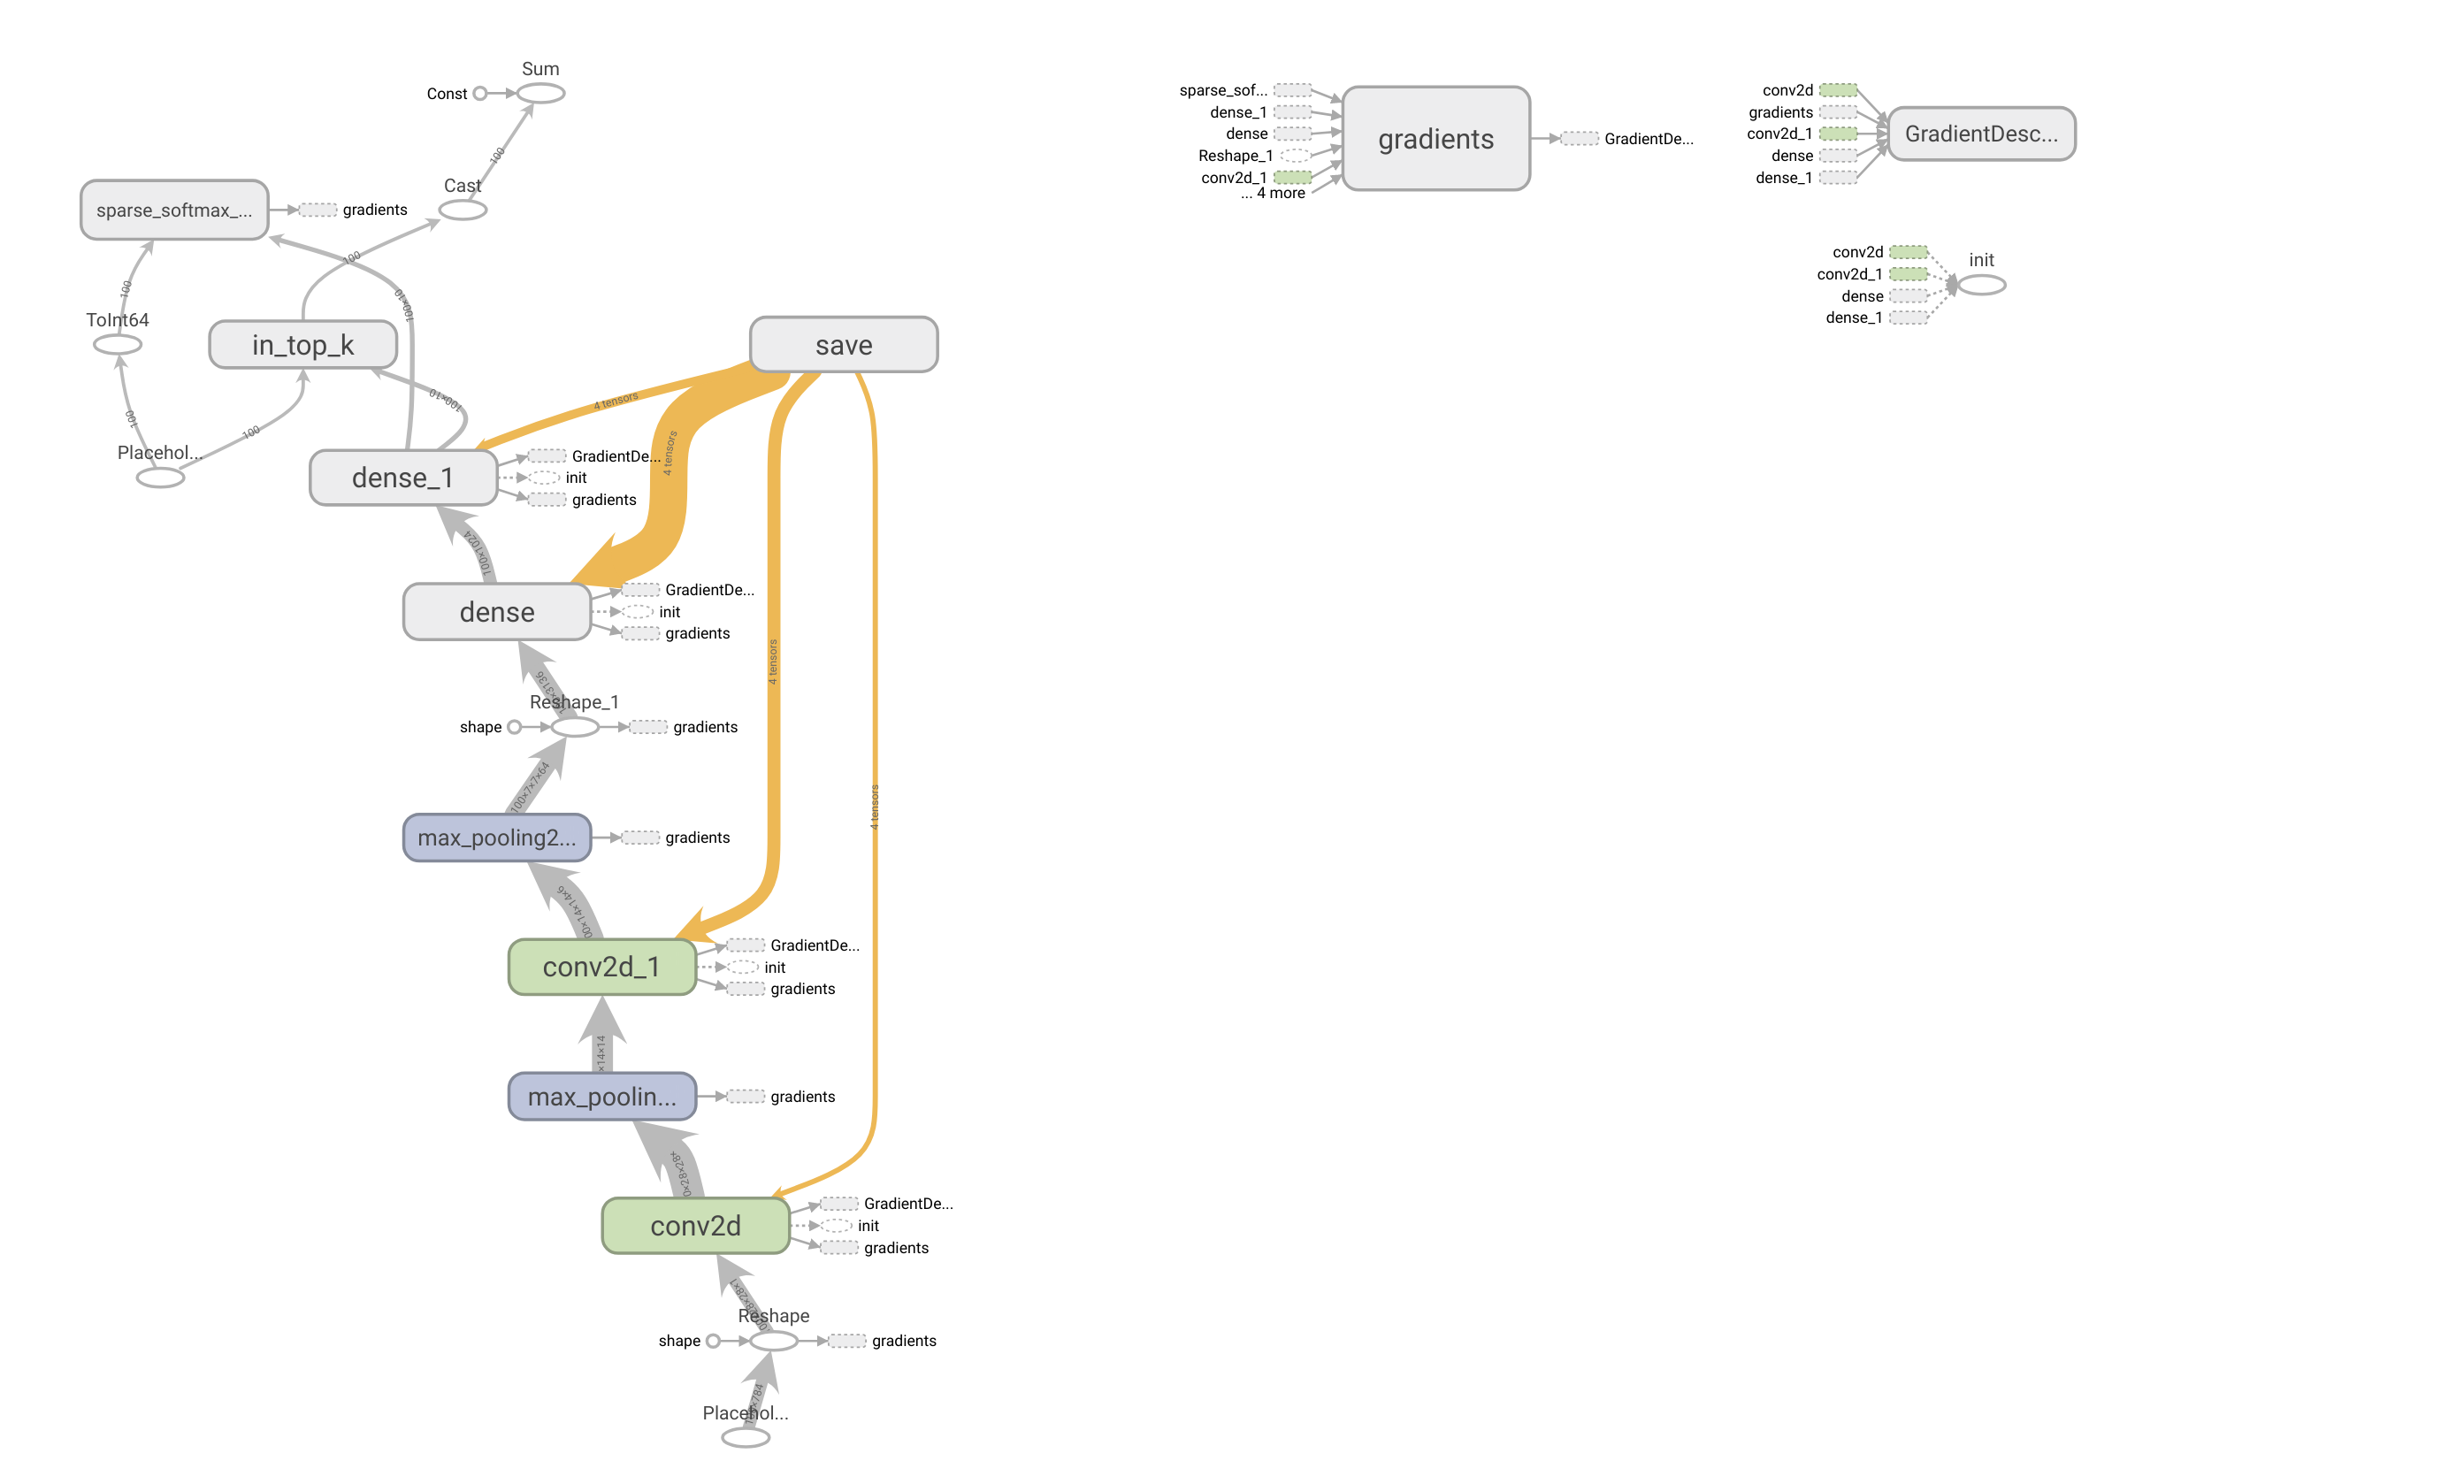
\includegraphics[width=\linewidth]{Graphs.png}
  \caption{Tensorboard : Structure Graphs}
  \label{fig:boat1}
\end{figure}
 

\begin{figure}
  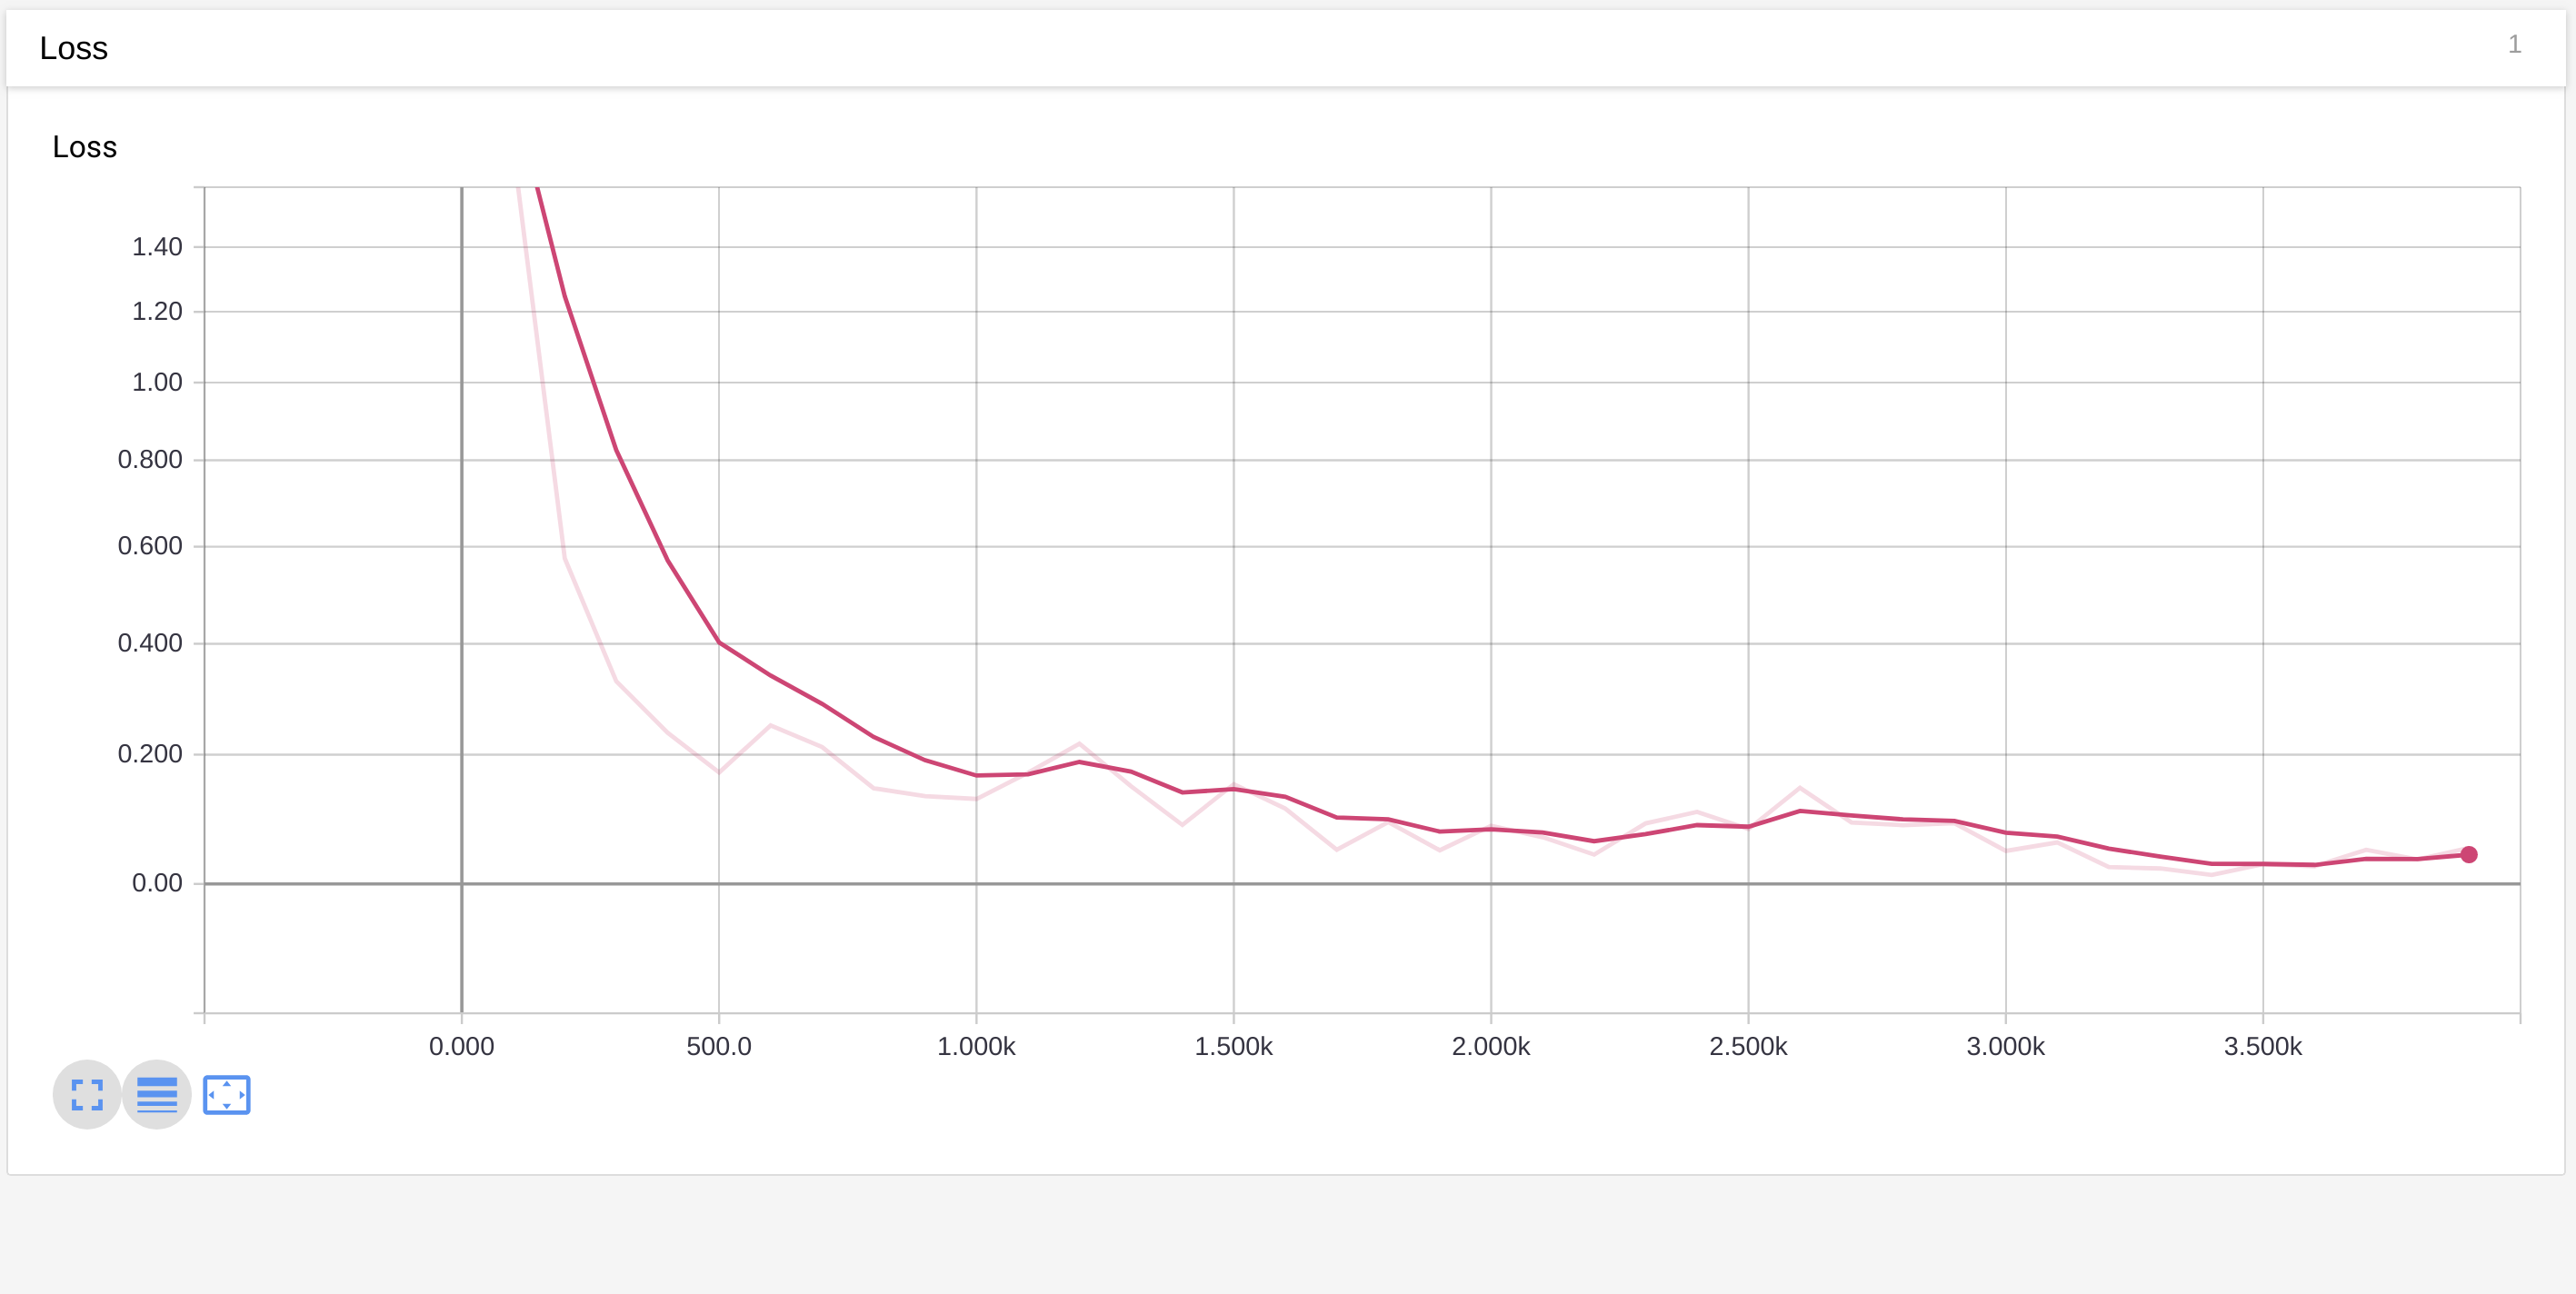
\includegraphics[width=\linewidth]{Loss.png}
  \caption{Tensorboard : Loss Over Time}
  \label{fig:boat1}
\end{figure}


\begin{figure}
  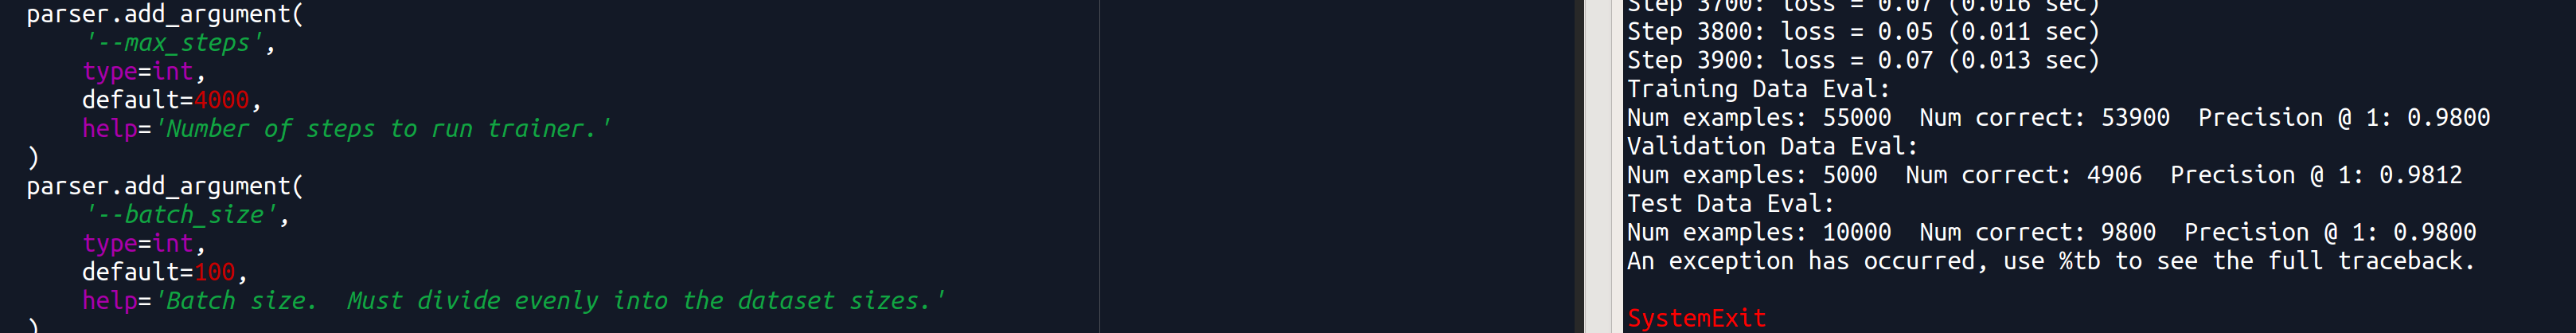
\includegraphics[width=\linewidth]{spyder-console.png}
  \caption{Console Results}
  \label{fig:boat1}
\end{figure}

	5.2 attach a short document describing the network architecture and any other architectures that you tested

	5.3 Make sure to have your full name and ID on the top of the document

	5.4 It is recommended to add tensorboard screenshots that describe the results (Optional)
	

\end{document}